\documentclass{report}

    \usepackage[latin1]{inputenc} %cool
    \usepackage[T1]{fontenc}
    \usepackage[english]{babel}
    \usepackage{blkarray}
    \usepackage{graphicx}
        
        \title{Computational Methods \\ Lab Session 1}
        \author{Augustin Reille}
        \date{2 october 2017}
        \begin{document}

        \maketitle
        \tableofcontents

            \section*{Abstract}
                In these lab sessions we had to use a C++ code to find the results of one 
                equation with two functions, using differents discretization schemes and compare them to the analytical solutions to see how the errors
                change. 
            \chapter{Introduction}
                In this first lab, we looked how the accuracy of a solution 
                of a linear equation was changing by using differents numerical
                schemes. \\
                We are considering the following problem : 
                \vspace{2mm}
                \[
                    \frac{\partial f}{\partial t}
                    + u \frac{\partial f}{\partial x} = 0
                \]
                \vspace{2mm}
                \[
                    x \in [\,-40, 40]\,
                \]
                \vspace{2mm}
                \[
                    u = 1    
                \]
                We have two functions to study, with boudaries conditions :
                \vspace{2mm}
                \[
                    f_{0} (x, 0) = 
                    \frac{1}{2} (sign(x) + 1)
                \]
                \vspace{2mm}
                \[
                    f_{0} (-40, t) = 0
                \]
                \vspace{2mm}
                \[
                    f_{0} (40, t) = 1
                \]
                and
                \vspace{2mm}
                \[
                    f_{1} (x, 0) = 
                    \frac{1}{2} exp(-x^{2})
                \]
                \vspace{2mm}
                \[
                    f_{1} (-40, t) = 0
                \]
                \vspace{2mm}
                \[
                    f_{1} (40, t) = 0
                \]

            \chapter{Methods}
                We want to solve the above problem with the initial conditions
    $f_{0}$ and $f_{1}$ on an uniform grid containing 100 points in $x$, using :
                \begin{itemize}
                    \item Upwind scheme
                    \item Central difference scheme
                    \item Lax scheme
                    \item Leapfrog scheme
                \end{itemize}
            \chapter{Results}
                \section*{Upwind scheme}
                    \section{Equations}
                        The upwind scheme corresponds to a discretisation with forward time and backward space.\\
                        We have :
                        \vspace{2mm}
                        \[
                            \frac{f_{i}^{n+1} - f_{i}^{n}}{\Delta t}
                            + a \frac{f_{i}^{n} - f_{i-1}^{n}}{\Delta x}
                            = 0
                        \]
                        \vspace{2mm}
                        \begin{equation}
                            \Leftrightarrow 
                            f_{i}^{n+1} = f_{i}^{n} (1 - a \frac{\Delta t}{\Delta x}) 
                            + a \frac{\Delta t}{\Delta x} f_{i-1}^{n}
                        \end{equation}

                    \section{Steps and Courant number}
                        Our study interval is $[\,-40, 40]\,$, so we have $80$ points.
                        We need to make our study over 100 points.\\
                        Our $\Delta x$ will be :
                        \vspace{2mm}
                        \[
                            \Delta x = \frac{80}{100} = 0,8
                        \]
                        To have a stable discretization scheme, we need to have our courant number $C$:
                        \vspace{2mm}
                        \[
                            C = u \frac{\Delta t}{\Delta x} < 1
                        \]
                        \vspace{2mm}
                        As we have $u = 1$, by taking $\Delta t = \Delta x / 2$, we will always have $C = 0,5 < 1$ .  (see Appendix A)

                    \section{Initialization and results calculation}

                        For each time value, we want the discrete solution for each of the 100 points of the interval.
                        Our matrix containing all results will look like :
                        \[
                            \begin{blockarray}{cccccc}
                            t_{0} & t_{1} & t_{2} & \cdots & t_{n} \\
                            \begin{block}{(ccccc)c}
                              a & b & c & \cdots & j & x_{0} \\
                              d & e & f & \cdots & k & x_{1} \\
                              g & h & i & \cdots & l & x_{2} \\
                              \vdots & \vdots & \vdots & \ddots & z & \vdots \\
                              w & x & y & \cdots & z & x_{i} \\
                            \end{block}
                            \end{blockarray}
                        \]
                        Here with the initial conditions we have, we are able to fullfill vectors $t_{0}$ and $x_{0}$. (see Appendix A)
                        Then, with equation $(3.1)$, we will be able to fullfill recursively the rest of the matrix, with a double for-loop (see Appendix B).
                        
                        \section{Graphical results and errors calcuation}
                        The red curve is the analytical solution, and the blue one is the one we get with the code. \\
                        We can see that the error increase with the time : if we take a value of a later time, the error will be bigger.
                        \begin{figure}[h]
                            \begin{center}
                            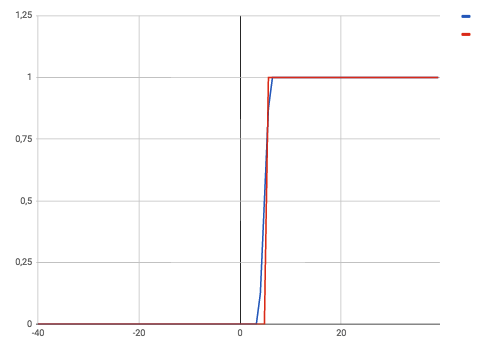
\includegraphics[width = 200px]{f0/t5/res.png} 
                            \end{center}
                            \caption{f0 with t = 5s}
                        \end{figure}
                        \begin{figure}[!h]
                            \begin{center}
                                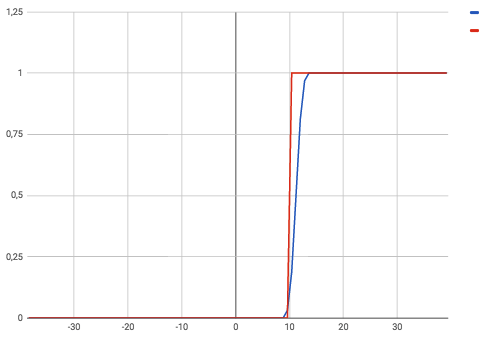
\includegraphics[width = 200px]{f0/t10/res.png} 
                            \end{center}
                            \caption{f0 with t = 10s}
                        \end{figure}
                        
                        \begin{figure}[!h]
                            \begin{center}
                            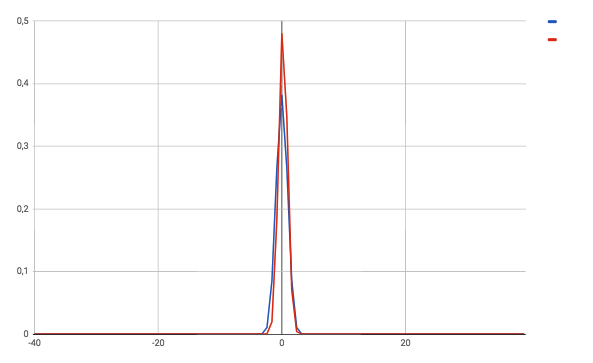
\includegraphics[width = 200px]{f1/t5/res.png} 
                            \end{center}
                            \caption{f1 with t = 5s}
                        \end{figure}
                        
                        \begin{figure}[h]
                            \begin{center}
                            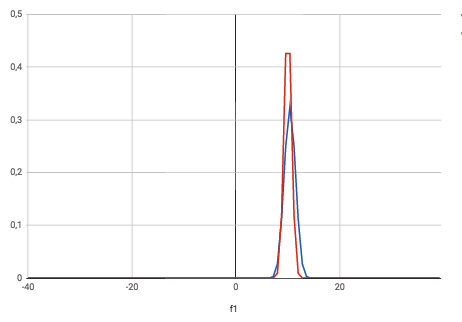
\includegraphics[width = 200px]{f1/t10/res.png} 
                            \end{center}
                            \caption{f1 with t = 10s}
                        \end{figure}
                \chapter{Discussion}
                    \section{Conclusion}
                        We see that in most of cases, the error increases with the time.
                        By doing a grid convergence study, and setting a grid with more points, we see that the error decrease; 
                        however the error is susceptible to increase locally due to computational errors (like truncation or calculation errors).
                    \section{Future work}
                        I only studied this grid convergence for the upwind scheme. I will have to make the study with the others schemes,
                        to see if they are more efficients, more stable with time and with a greater number of mesh points.

                \chapter{Appendices}
                \newpage
                    \section{Appendix A : initialization}
                    C++ code to initialize our result table
                    \begin{verbatim}
int nspace = 100;
int tottime = 22;
double dx = 0.8;
double dt = dx / 2;
int ntime = tottime / dt;
double courantNumber = dt / dx;

// the vector containing our results :
double results[ntime][nspace];

/* initial conditions
* here is the code for f1 only
*/
for (int i = 0; i < nspace; i++)
{
    double x = -40 + i * dx;
    results[0][i] = 0.5 * exp(-(x * x));
}
for (int n = 0; n < ntime; n++)
{
    results[n][0] = 0;
    results[n][nspace - 1] = 0;
}
                    \end{verbatim}
                \section{Appendix B : the double for-loop}

                C++ code to fullfill our result table
                    \begin{verbatim}
// loop
for (int n = 1; n < ntime; n++)
{
    for (int i = 1; i < nspace - 1; i++)
    {
        results[n][i] = results[n - 1][i] * (1 - courantNumber) 
                        + courantNumber * results[n - 1][i - 1];
    }
}
                    \end{verbatim}

        \end{document}